\documentclass[a4paper,12pt,twocolumn]{article}
\usepackage[english]{babel}
\usepackage{times}
\usepackage{setspace}
\usepackage{inputenc}
\usepackage{amssymb}
\usepackage{amsfonts}
\usepackage[pdftex]{graphicx}
\usepackage{subfigure}
\usepackage{alltt}
\usepackage{moreverb}
%for more info on hyperref package see http://en.wikibooks.org/wiki/LaTeX/Packages/Hyperref
\usepackage[pdftex,colorlinks=true,linkcolor=blue]{hyperref}
\usepackage{eso-pic}
\setlength{\columnsep}{3em}

\usepackage{geometry}
%\geometry{hmargin={30mm,15mm},vmargin={26mm,26mm}}
%\geometry{total={14cm,20.5cm},includehead}
\geometry{hmargin={20mm,20mm},vmargin={20mm,20mm}}
\geometry{mag=1414}

\newcommand\BackgroundPic{
\put(-15,0){
\parbox[b][\paperheight]{\paperwidth}{%
\vfill
\centering
  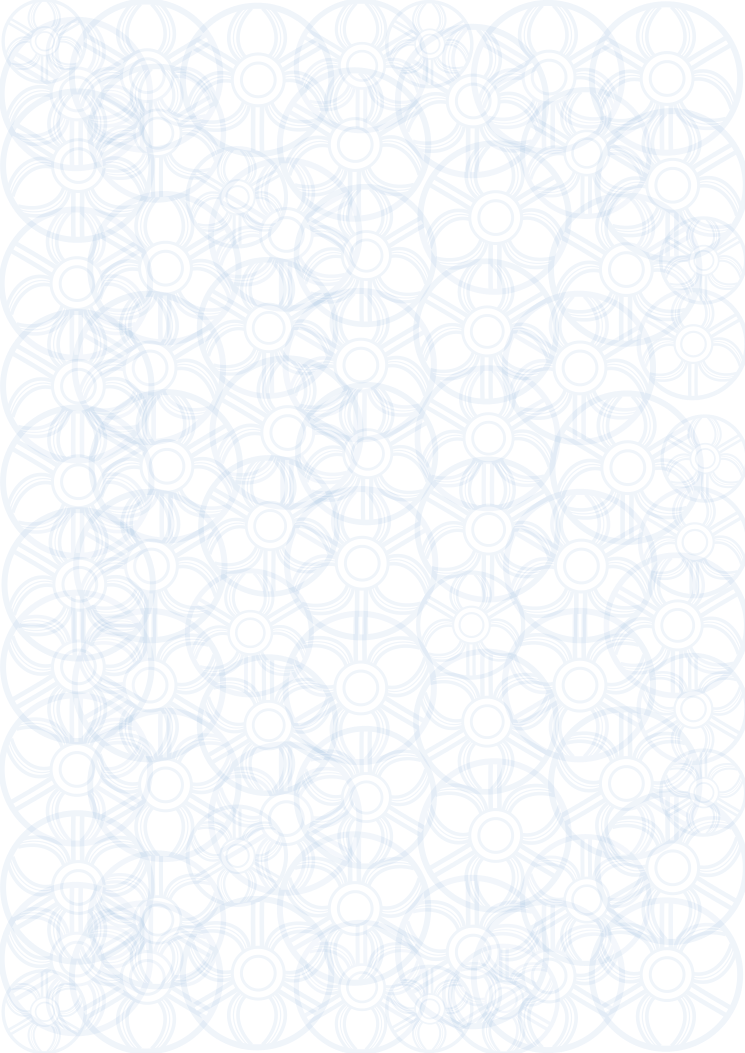
\includegraphics[width=1.1\paperwidth,height=1.1\paperheight, keepaspectratio]{images/00-background.png}%
\vfill
}}}

\begin{document}
\AddToShipoutPicture{\BackgroundPic}
\subsection*{What is TG?}
  Trident Genesis is a pure Java software platform for agile development of information systems in a domain-centric way.
  It addresses all aspects of application development: data tier, logic tier and presentation tier.

\subsubsection*{Domain Driven Design}
  Software architecture can be reused. 
  Domain architecture is very often unique (customer specific).
  Modeling of the business domain is the core value for customers.
  TG Platform encapsulates the complexity of the software architecture and emphasises the domain architecture.
  \\ \\
  \noindent The typical development workflow includes: modeling of business domain (ontological aspect), implement core business rules and configure the user interface.
  These steps are facilitated by high level abstractions provided by the platform, which handles the low level technical details automatically.
  Thus, the platform enables developers to concentrate on the modeling of the business domain ensuring higher productivity and quality of the final product.


 \subsection*{Core features and principles}
  TG is designed to ensure that the application is easy to use and incorporates the following principles and technologies:

  \begin{itemize}
    \item Domain centric application development with a life cycle revolving around business entities and logic.
    \item Fully resource oriented architecture (ROA).
    \item Excellent performance scalability (both horizontally and vertically).
    \item TG-based applications are automatically Rich Internet applications (RIA)
    \item Secure -- utilises Amazon S3 like approach to authentication.
    \item Pluggable authorisation model (e.g. LDAP, DB-based), declarative security.
    \item High level degree of configuration.
    \item Intensive utilisation of declarative and meta programming.    
    \item Ease of user interface (UI) construction in a domain centric way while provisioning ways for high interactivity.
    \item Domain Query API (provides object-oriented means to query persisted domain entities) with built-in visual composer (Snappy).
    \item RDBMS independent.
    \item Data auditing and role-based data visibility control.
    \item Support for separation of development roles (domain logic and UI can be developed concurrently).
  \end{itemize}

  \begin{figure}[!h]
  \centering
  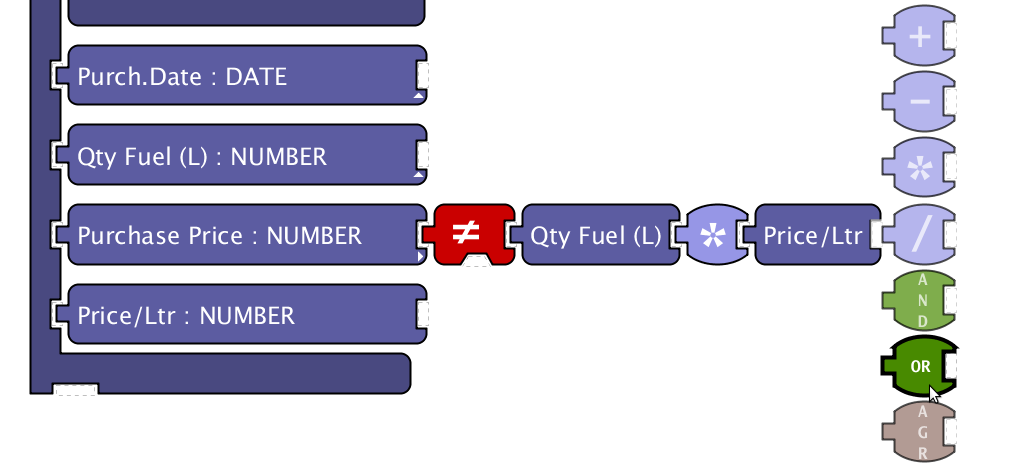
\includegraphics[scale=0.22]{images/01-rulesarea-suggestionmenu.png}  
  \end{figure}

\subsection*{Main advantages}
  \begin{itemize}
    \item Pure Java, which reduces the learning curve (no need to know HTML, CSS, JavaScript and other browser-related technologies).
    \item Entry level development skills requirement.
    \item Improves application maintainability: code is limited mostly to domain definition and business logic.
    \item Increases speed of development.
    \item Applications are RIA/ROA.
    \item Covers a complete development life cycle -- from DB to UI.
    \item OS and RDBMS independent.
    \item Ensures data integrity automatically.
    \item Ready to be extended by 3rd party developers if required.
  \end{itemize}

\subsection*{Designed for ease of use and learning by end-users}
 
\subsubsection*{Intuitive}
  From constant communication with customers, Fielden understands how their applications are utilised. 
  We incorporate this understanding into the ways TG-based applications are designed covering task flows and features that are essential at key points within the user experience, making the application extremely intuitive.
  Applications always provide a sensible feedback to the user in non-intrusive ways reducing the confusion and disruption of the workflow.
  \begin{figure}[!h]
  \centering
  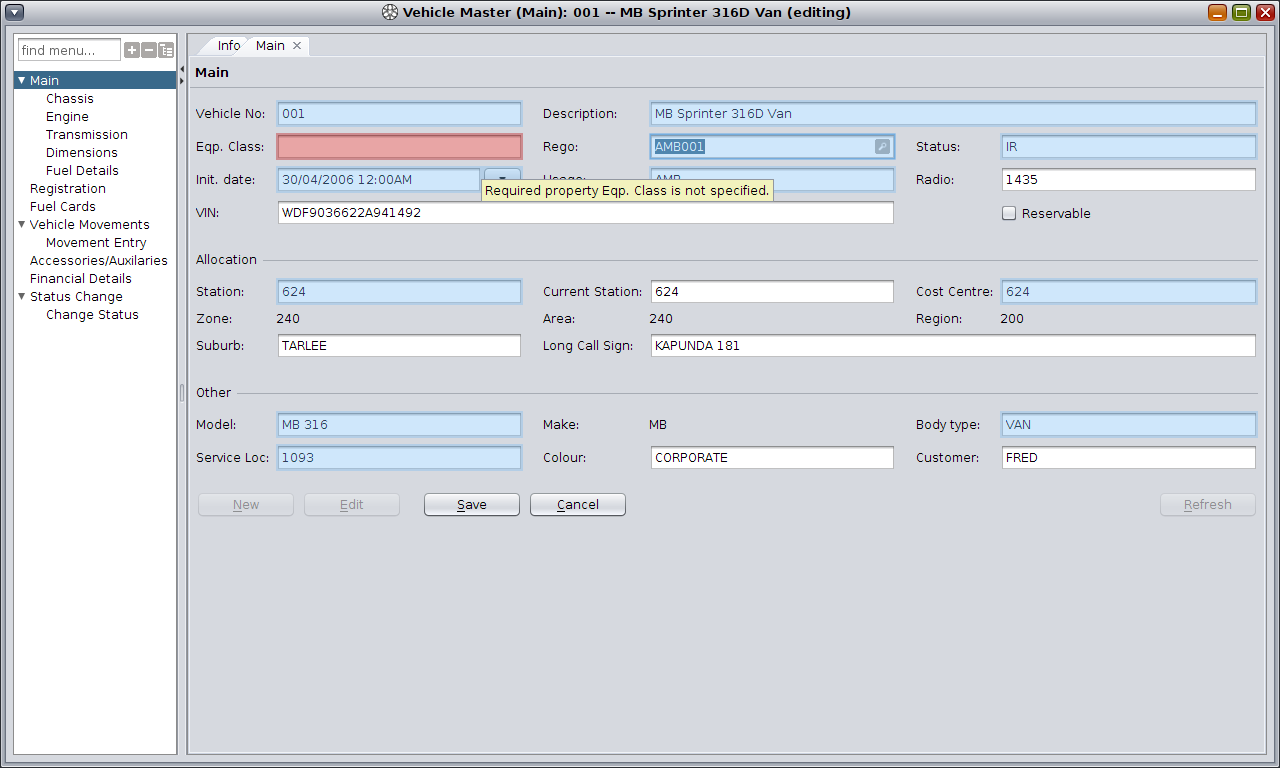
\includegraphics[scale=0.17]{images/04-veh-master-main-error.png}
  \end{figure}

\subsubsection*{Consistency}

  Consistency makes software easier to use. 
  Things that look the same should behave in a consistent fashion, and an action should always produce the same result. 
  In TG-based applications, all UI elements that look the same -- operate the same way. 
  The platform provides the highest level of consistency across all parts of the application to quickly move from function to function, without confusion and wasted effort.
 
\subsubsection*{Flexibility}
  Recognizing that every customer and every user is different, TG platform is designed to provide high flexiblity of the end product. 
  Organisations using TG-based solutions do not have to change processes or terminology -- their domain is fully reflected in the application. 
  Users can customize the application to meet their unique needs.
  The administrative function provides easy ways to configure and customise access to the features that users should access based on their role.

  \begin{figure}[!h]
  \centering
  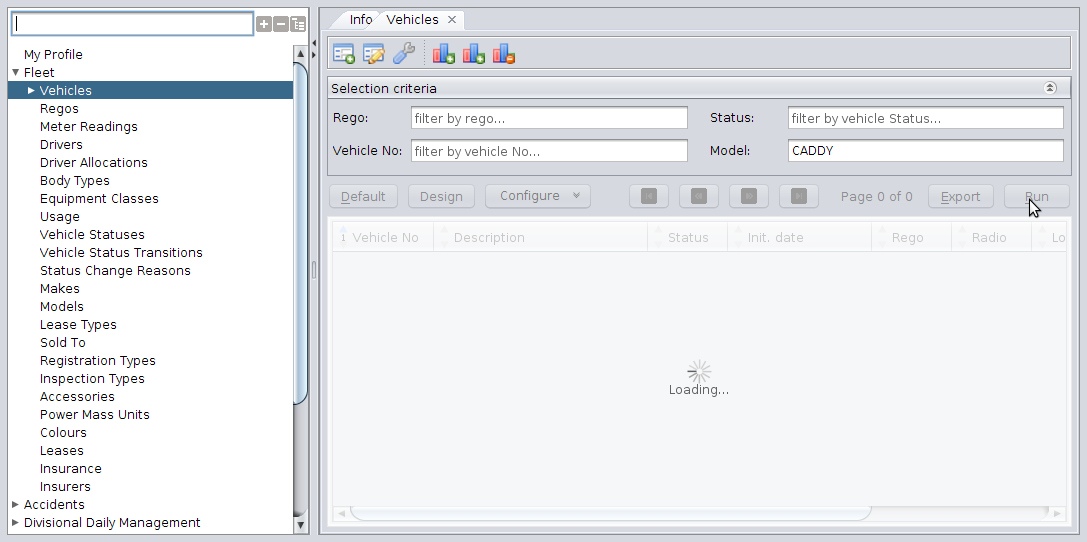
\includegraphics[scale=0.2]{images/03-running.png}
  \end{figure}

\subsubsection*{Interactivity}
  TG-based applications utilise the full potential and richness of the desktop UI providing users with highly interactive experience.
  The platform incorporates the implementation of the Zooming User Interface paradigm, which provides support for integration with Scalable Vector Graphics files.

  \begin{figure}[!h]
  \centering
  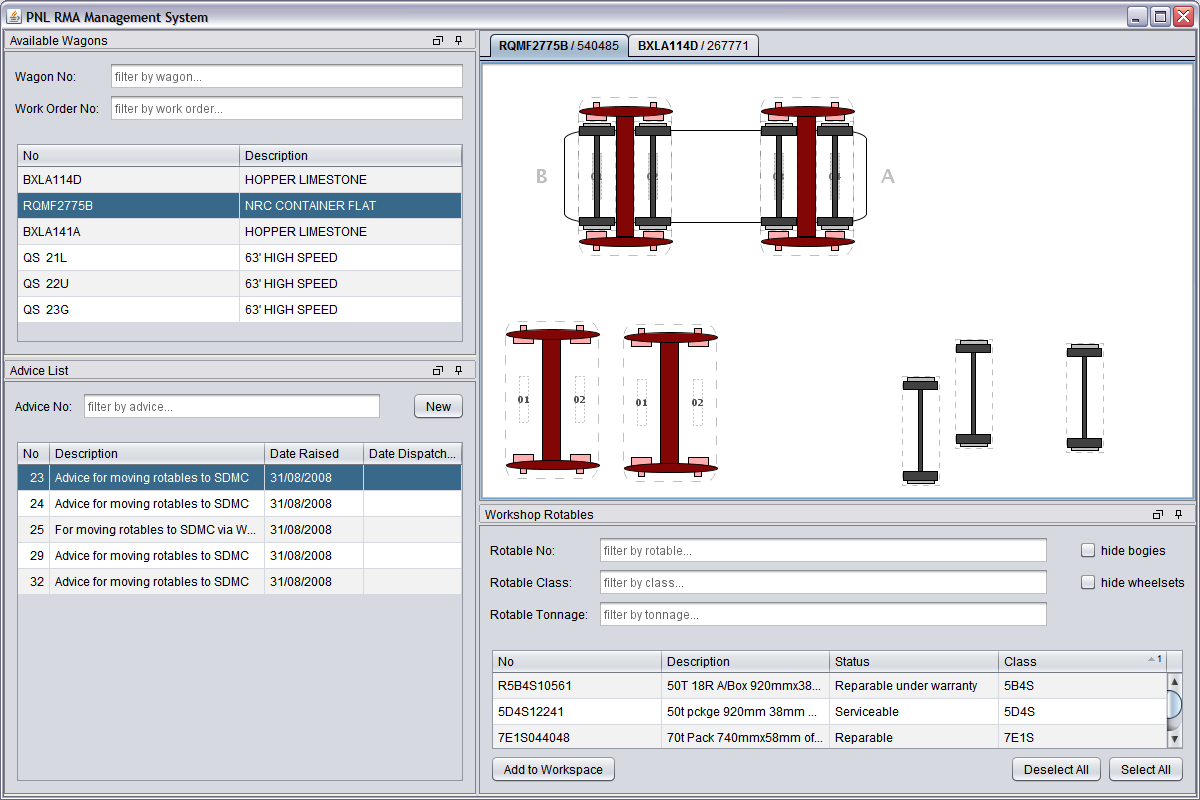
\includegraphics[scale=0.18]{images/02-workspace-custom-layout.png}
  \end{figure}

\end{document}

